
\documentclass{bredelebeamer}
\usepackage{textcomp}
\usepackage[utf8]{inputenc}
\usepackage[T1]{fontenc}
\usepackage{helvet}
\usepackage{wrapfig}
\usepackage{graphicx}
\graphicspath{ {images/} }
\usepackage{ragged2e}
%\usepackage[main=english, french]{babel}

\AtBeginSection[]
{
  \begin{frame}<beamer>
    \frametitle{Part \thesection}
    \tableofcontents[currentsection]
  \end{frame}
}


%%%%%%%%%%%%%%%%%%%%%%%%%%%%%%%%%%%%%%%%%%%%%%%%



\title[Long Project with Audiogaming]{Long Project with Audiogaming}
% Titre du diaporama

\subtitle{Additive Synthesis with Inverse Fourier Transform for Non-Stationary Signals }
% Sous-titre optionnel

\author{ \hspace{0.3cm} C. Cazorla - V. Chrun - B. Fundaro - C. Maliet \hspace{0.3cm} }
% La commande \inst{...} Permet d'afficher l' affiliation de l'intervenant.
% Si il y a plusieurs intervenants: Marcel Dupont\inst{1}, Roger Durand\inst{2}
% Il suffit alors d'ajouter un autre institut sur le modèle ci-dessous.

\institute[Audiogaming Supervisor ]
{
  \normalsize Audiogaming Supervisor : \\
 \normalsize Chunghsin Yeh
  }


\date{March 03, 2017}
% Optionnel. La date, généralement celle du jour de la conférence

\subject{Long Project with Audiogaming}
% C'est utilisé dans les métadonnes du PDF


\logo{
\includegraphics[scale=0.08]{enseeiht.png}
%\includegraphics[scale=0.15]{ag.png}
}



%%%%%%%%%%%%%%%%%%%%%%%%%%%%%%%%%%%%%%%%%%%%%%%%%%%%%%%%%%%%%%%%%%%%%
\begin{document}

\begin{frame}
  \titlepage
\end{frame}


%%%%%%%%%%%%%%%%%


\begin{frame}{Content}
  \tableofcontents
\end{frame}

%-------------------------------------------------------
\section{Introduction}
%-------------------------------------------------------
\subsection{The company}
\begin{frame}{Introduction}{The company}
%-------------------------------------------------------
	\begin{figure}
   	 \centering
  	 \includegraphics[scale=0.12]{ag.png}
	 \end{figure}
  \begin{itemize}
  \item<1-> Localization: Toulouse, Paris
  \item<1-> Activity: Audio plug-in (VSTs and RTAS)
  \item<1-> Main customers: Film and Video Game Industry (Sony, Ubisoft)
  \item<1-> 10 employees
	\begin{figure}
	\includegraphics[scale=0.12]{AudioFire_screen.png}
	\caption{Audiofire: audio plug-in that recreates fire sound}
	\end{figure}
  \end{itemize}
\end{frame}

%-------------------------------------------------------
\subsection{Objective}
\begin{frame}{Introduction}{Objective}
%-------------------------------------------------------


  \begin{itemize}
          \item<1-> We are continuing the Audiogaming long project from 2015 (Emilie Abia, Lili Zheng, Quentin Biache)
\begin{block}{}
\begin{center} {\it Objective} : Synthesizing sounds from their spectrum with a $ FFT^{-1} $ \end{center}
	\begin{figure}
	\includegraphics[scale=0.4]{Analysis_Synthesis.png}
	\caption{General approach for modifying a sound in the spectral domain}
	\end{figure}
\end{block}   
	\item<1-> We have to implement a new method of additive synthesis $\Rightarrow$ computationally very fast
  \end{itemize}
\end{frame}

%-------------------------------------------------------
\subsection{Context of the Project}
\begin{frame}{Introduction}{Context of the Project}
%-------------------------------------------------------

  \begin{itemize}
    \item<1-> 6 weeks only $\Rightarrow$ Focus on the synthesis method only.
   \begin{block}{}
	 Given codes in Python and Matlab from the 2015 project :
   \begin{itemize}
 	\item<1-> Python : Analysis estimator of sinus parameters and sinus generation with those parameters (only stationary)
 	\item<1-> Matlab : Some reasearch on the Non-stationary synthesis with the LUT of lobes
   \end{itemize}
   \end{block}   
	\item<1-> We made our own Object Oriented Programmation tree structure in Python
	\item<1-> We remade all the codes to be coherent with the OOP tree structure
  \end{itemize}
\end{frame}

%-------------------------------------------------------
\subsection{Work Environment and Project Management}
\begin{frame}{Introduction}{Work Environment}
%-------------------------------------------------------

\begin{figure}
	\centering
	\includegraphics[scale=0.4]{all_softwares.png}
	\caption{ {\it PyCharm} as Python IDE , {\it Slack} to communicate,{\it GitHub} to stock the codes and have a versionning, {\it Freedcamp} to plan the project events }
\end{figure}
\end{frame}

\begin{frame}{Introduction}{Project Management : Gantt Chart (expected event)}
%-------------------------------------------------------

\begin{figure}
	\centerline{\includegraphics[scale=0.28]{Gantt.png}}
\end{figure}
\end{frame}

\begin{frame}{Introduction}{Project Management : Gantt Chart now}
%-------------------------------------------------------

\begin{figure}
	\centerline{\includegraphics[scale=0.28]{Gantt2.png}}
\end{figure}
\end{frame}

%%%%%%%%%%%%%%%%%
%-------------------------------------------------------
\section{Method Overview}
%-------------------------------------------------------
\subsection{Additive Synthesis (Time Domain)}
\begin{frame}{Additive Synthesis}{Time Domain}
%-------------------------------------------------------
\begin{block}{}
The sound signal is represented as a sum of N sinusoids: \\
\centerline{
$ x(t) = \sum\limits_{n=1}^N a_{n} sin(2 \pi f_{n} t + \phi_{n})$}
\begin{itemize}
\item Very costly to implement
\item Impossible to compute in real-time
\end{itemize}
\end{block}
\begin{figure}
	\centerline
	{\includegraphics[scale=0.25]{additif.png}}
	\caption{\it The additive synthesis}
\end{figure}
\end{frame}

%-------------------------------------------------------
\subsection{Method Overview}
\begin{frame}{Method Overview : Windowing}{Analysis}
%-------------------------------------------------------
\begin{figure}
	\centerline
	{\includegraphics[scale=0.4]{slide1.png}}
	\caption{\it Windowing step}
\end{figure}
\end{frame}

\begin{frame}{Method Overview : Peak detection in Frequency Domain}{Analysis}
%-------------------------------------------------------
Peak detection and extraction of parameters by STPT (particular Short Time Fourier Transform):
\begin{figure}
	\centerline
	{\includegraphics[scale=0.5]{slide2.png}}
	\caption{\it Peak detection}
\end{figure}
\end{frame}

\begin{frame}{Method Overview : Result ( FFT$^{-1}$)}{Synthesis}
%-------------------------------------------------------
Additive synthesis with FFT$^{-1}$ according to the parameters from the analysis:
\begin{figure}
	\centerline
	{\includegraphics[scale=0.5]{synthesisstep.png}}
	\caption{\it Synthesized frame vs Original frame}
\end{figure}
\end{frame}


%%%%%%%%%%%%%%%%%
%-------------------------------------------------------
\section{The additive synthesis in frequency domain}
%-------------------------------------------------------
\subsection{Stationary Case}
\begin{frame}{Stationary Case}{Stationary sinusoidal model}
%-------------------------------------------------------
\begin{block}{Mathematical model  :}

\begin{equation}
s(t) = a_0 exp[j(2 \pi f_0 t + \phi_0)]
\end{equation}
\end{block}
\begin{itemize}
\item 3 parameters: $a_0$ (amplitude), $f_0$ (frequency) and $\phi_0$ (phase).
\item Simplest model but useful for certain kinds of signals.
\item Each spectral bin represents a stationary sinusoid.
\item $\Rightarrow$ generate a synthetic spectrum with the desired parameters\\ $\Rightarrow$ generate a main lobe derived from the Fourier transform of the normalized window $w$ supposedly\footnote{Because no actual analysis happened} used during analysis \\ $\Rightarrow$ place it at the right position on the spectrum.
\end{itemize}

\end{frame}
%-------------------------------------------------------
\begin{frame}{Stationary Case}{Lobe generation}
%-------------------------------------------------------
\begin{block}{}
We generate the sinusoids in frequency domain : \\

\begin{itemize}
\item Window the signal to maximize the energy in the main lobe
\item We only keep the main lobe for each sine (11 points)
\item We assume that the parameters (amplitude, frequency, phase) are already given by the analysis
\item We interpolate the relevant bins value if by any chance the wanted frequency $\hat{f}$ is not exactly on a bin, that is to say if $\hat{f} \notin \{\frac{2 k \pi}{N} \}_{k=0...N-1}$
\end{itemize}
\end{block}
\begin{figure}
	\centerline
	{\includegraphics[scale=0.45]{lobe.png}}
	\caption{\it Windowed sine lobe}
\end{figure}
\end{frame}
%-------------------------------------------------------
\begin{frame}{Stationary Case}{Frames separation}
%-------------------------------------------------------

The sound signal is  a frame-by-frame signal: \\
The analysis hop size will be called $R_a$ and the synthesis hop size $R_s$ (moving step of the frame)
\begin{figure}

	{\includegraphics[scale=0.25]{overlap2.png}}
	\caption{\it Sum of small size Hanning windows}
\end{figure}
\begin{figure}
	{\includegraphics[scale=0.25]{overlap1.png}}
	\caption{\it Overlap and add}
\end{figure}
\end{frame}
%-------------------------------------------------------
\begin{frame}{Stationary Case}{Phase Coherence}
%-------------------------------------------------------

\begin{block}{Phase coherence}
The Phase coherence is not a problem in the Stationary case :
\begin{itemize}
\item We don't know the window effect on the phase : ${f_{w, \hat{f}}(\phi) : \phi \mapsto \tilde{\phi}}$  \\
$ \Rightarrow$ We calculate its influence on the first frame and assume the same influence on the other frame.

\item We then multiply the generated lobe by $\frac{A}{2}$ and set the lobe phase to $\tilde{\phi} + 2\pi \hat{f} R_a$   
\item In the purely stationary case, the expected phase shift is the theoretical phase shift :

\begin{equation}
\begin{cases}
\tilde{\phi}_i = \tilde{\phi}_{i-1} + 2\pi \hat{f} R_a \\
\tilde{\phi}_0 = \tilde{\phi}
\end{cases}
\end{equation}

\end{itemize}
\end{block}


\end{frame}
%-------------------------------------------------------
\subsection{Quasi-Stationary Case}
\begin{frame}{Quasi-Stationary Case}{What is changing}
%-------------------------------------------------------
\begin{itemize}
\item In a Quasi-stationary case, the sine wave can change a little bit in frequency. \\
 Main problem $\Rightarrow$ Phase coherence !
\item We need to implement a a method to correct the phase : Phase Vocoder !
\end{itemize}

\begin{figure}
{\includegraphics[scale=0.45]{pvoverview.png}}
	\caption{\it Phase Vocoder overview}
\end{figure}


\end{frame}
%-------------------------------------------------------
\begin{frame}{Quasi-Stationary Case}{What is changing}
%-------------------------------------------------------
\begin{itemize}
\item In a Quasi-stationary case, the sine wave can change a little bit in frequency. \\
 Main problem $\Rightarrow$ Phase coherence !
\item We need to implement a a method to correct the phase : Phase Vocoder !
\end{itemize}

\begin{block}{Phase Vocoder}
In this case, the phase changing is different from the stationary case.
We have to calculate the instantaneous frequency for the kth bin:
\begin{equation}
\hat{\omega}_{k} (t_{a}^{u})= \Omega_{k} + \frac {\Delta_{p} \Phi_{k}^{u}} {R_{a}}
\end{equation}
\centering
Where:
\begin{equation}
\Delta\Phi_{k}^{u} = \angle X(t_{a}^{u}, \Omega_{k}) - \angle X(t_{a}^{u-1}, \Omega_{k}) - R_{a}\Omega_{k}
\end{equation}
\centering
Hence,
\begin{equation}
\angle Y(t_{s}^{u}, \Omega_{k}) = \angle Y(t_{s}^{u-1}, \Omega_{k}) + R_{s}\hat{\omega}_{k}(t_{a}^{u})
\end{equation}

We replace the output signal phase by this one.
\end{block}

\end{frame}
%-------------------------------------------------------
\subsection{Non-Stationary Case}
\begin{frame}{Non-Stationary Case}{A different approach}
%-------------------------------------------------------

\begin{block}{Mathematical model  :}

\begin{equation}
s(t) = exp[(\lambda_0 + \mu_0 t) + j(\phi_0 + 2\pi f_0 t + \frac{\psi_0}2 t^2 )]
\end{equation}
\end{block}
\begin{itemize}
\item 5 parameters: \\ $(\lambda_0 + \mu_0 t)$ (overall amplitude)\\ $f_0$ (frequency)\\ $\phi_0$ (phase) \\ $ \mu_0$ (amplitude change rate (ACR))\\ $\psi_0$ (frequency change rate (FCR))
\item The analysis part give us all those parameters
\item To manage the influence of the ACR and the FCR on the lobe $\Rightarrow$ Interpolation of Look-up table of already saved lobes with different (ACR,FCR).
\end{itemize}

\end{frame}
%-------------------------------------------------------
\begin{frame}{Non-Stationary Case}{Look up table}
%-------------------------------------------------------
\begin{figure}
   \begin{minipage}[c]{.46\linewidth}
      \includegraphics[scale=0.3]{grid.png}
      \caption{\it ACR/FCR grid}
   \end{minipage} \hfill
   \begin{minipage}[c]{.46\linewidth}
      \includegraphics[scale=0.35]{LUT.png}
      \caption{\it Look-up table}
   \end{minipage}
\end{figure}

\end{frame}

%-------------------------------------------------------
\begin{frame}{Non-Stationary Case}{Phase Vocoder : Scaled-Phase Locking}
%-------------------------------------------------------
\begin{itemize}
\item We can use the phase vocoder to correct the phase, but the main problem is sine waves that switch from a frequency bin to another bin. The phase might change a lot from one frame to another.
\item $\Rightarrow$ We use a refined version of the phase vocoder : Scaled-Phase Locking \\
 $\Rightarrow$ It takes into account the frequency trajectory of each lobes.
\begin{figure}
      \includegraphics[scale=0.4]{peaktrajectory.png}
      \caption{\it Peak coherence from a frame to another}
\end{figure}
\end{itemize}

\end{frame}
%-------------------------------------------------------
\begin{frame}{Non-Stationary Case}{Phase Vocoder : Scaled-Phase Locking}
%-------------------------------------------------------
\begin{block}{ Scaled-Phase Locking}
We find each region corresponding to each peaks, and then we use the phase vocoder algorithm for each region :\\
$k_0$ is the precedent frequency bin for the peak - $k_1$ is the current frame peak bin :
\begin{equation}
\hat{\omega}_{k_1} (t_{a}^{u})= \Omega_{k} + \frac {\Delta_{p} \Phi_{k}^{u}} {R_{a}}
\end{equation}
\centering
Where:
\begin{equation}
\Delta\Phi_{k_1}^{u} = \angle X(t_{a}^{u}, \Omega_{k_1}) - \angle X(t_{a}^{u-1}, \Omega_{k_0}) - R_{a}\Omega_{k_1}
\end{equation}
\centering
Hence,
\begin{equation}
\angle Y(t_{s}^{u}, \Omega_{k_1}) = \angle Y(t_{s}^{u-1}, \Omega_{k_0}) + R_{s}\hat{\omega}_{k_1}(t_{a}^{u})
\end{equation}
\centering 
Then for each bin in the region :
\begin{equation}
\angle Y(t_{s}^{u}, \Omega_{k}) = \angle Y(t_{s}^{u}, \Omega_{k_1}) + \beta [ \angle X(t_{a}^{u}, \Omega_{k}) - \angle X(t_{a}^{u}, \Omega_{k_1}) ]
\end{equation}
\end{block}


\end{frame}
%-------------------------------------------------------
\begin{frame}{Non-Stationary Case}{Scaled-Phase Locking Problem}
%-------------------------------------------------------
\begin{itemize}
\item Moreover, we do not know for now how to manage the peaks that appear and disappear
\begin{figure}
      \includegraphics[scale=0.5]{phaselocking.png}
      \caption{\it Phase-locking problem}
\end{figure}
\end{itemize}

\end{frame}


%%%%%%%%%%%%%%%%%
%-------------------------------------------------------
\section{Result}
%-------------------------------------------------------
\subsection{Stationary Case}
\begin{frame}{Stationary Case}{Protocol}
%-------------------------------------------------------
\begin{itemize}
\item A one second triangular signal consisting in 84 frames
\item We first vary the number of harmonics and compare the time of execution
\item In a second time, for a 10 harmonics signal, we vary the frequency and investigate the reconstruction error.
\end{itemize}
\end{frame}
%-------------------------------------------------------
\begin{frame}{Stationary Case}{Triangular wave synthesis}
%-------------------------------------------------------
\begin{figure}
      \includegraphics[scale=0.15]{triangle.png}
      \caption{\it original vs. synthesized triangular wave}
\end{figure}
\end{frame}
%-------------------------------------------------------
\begin{frame}{Stationary Case}{Time and Relative-Time}
%-------------------------------------------------------
\begin{figure}
   \begin{minipage}[c]{.46\linewidth}
      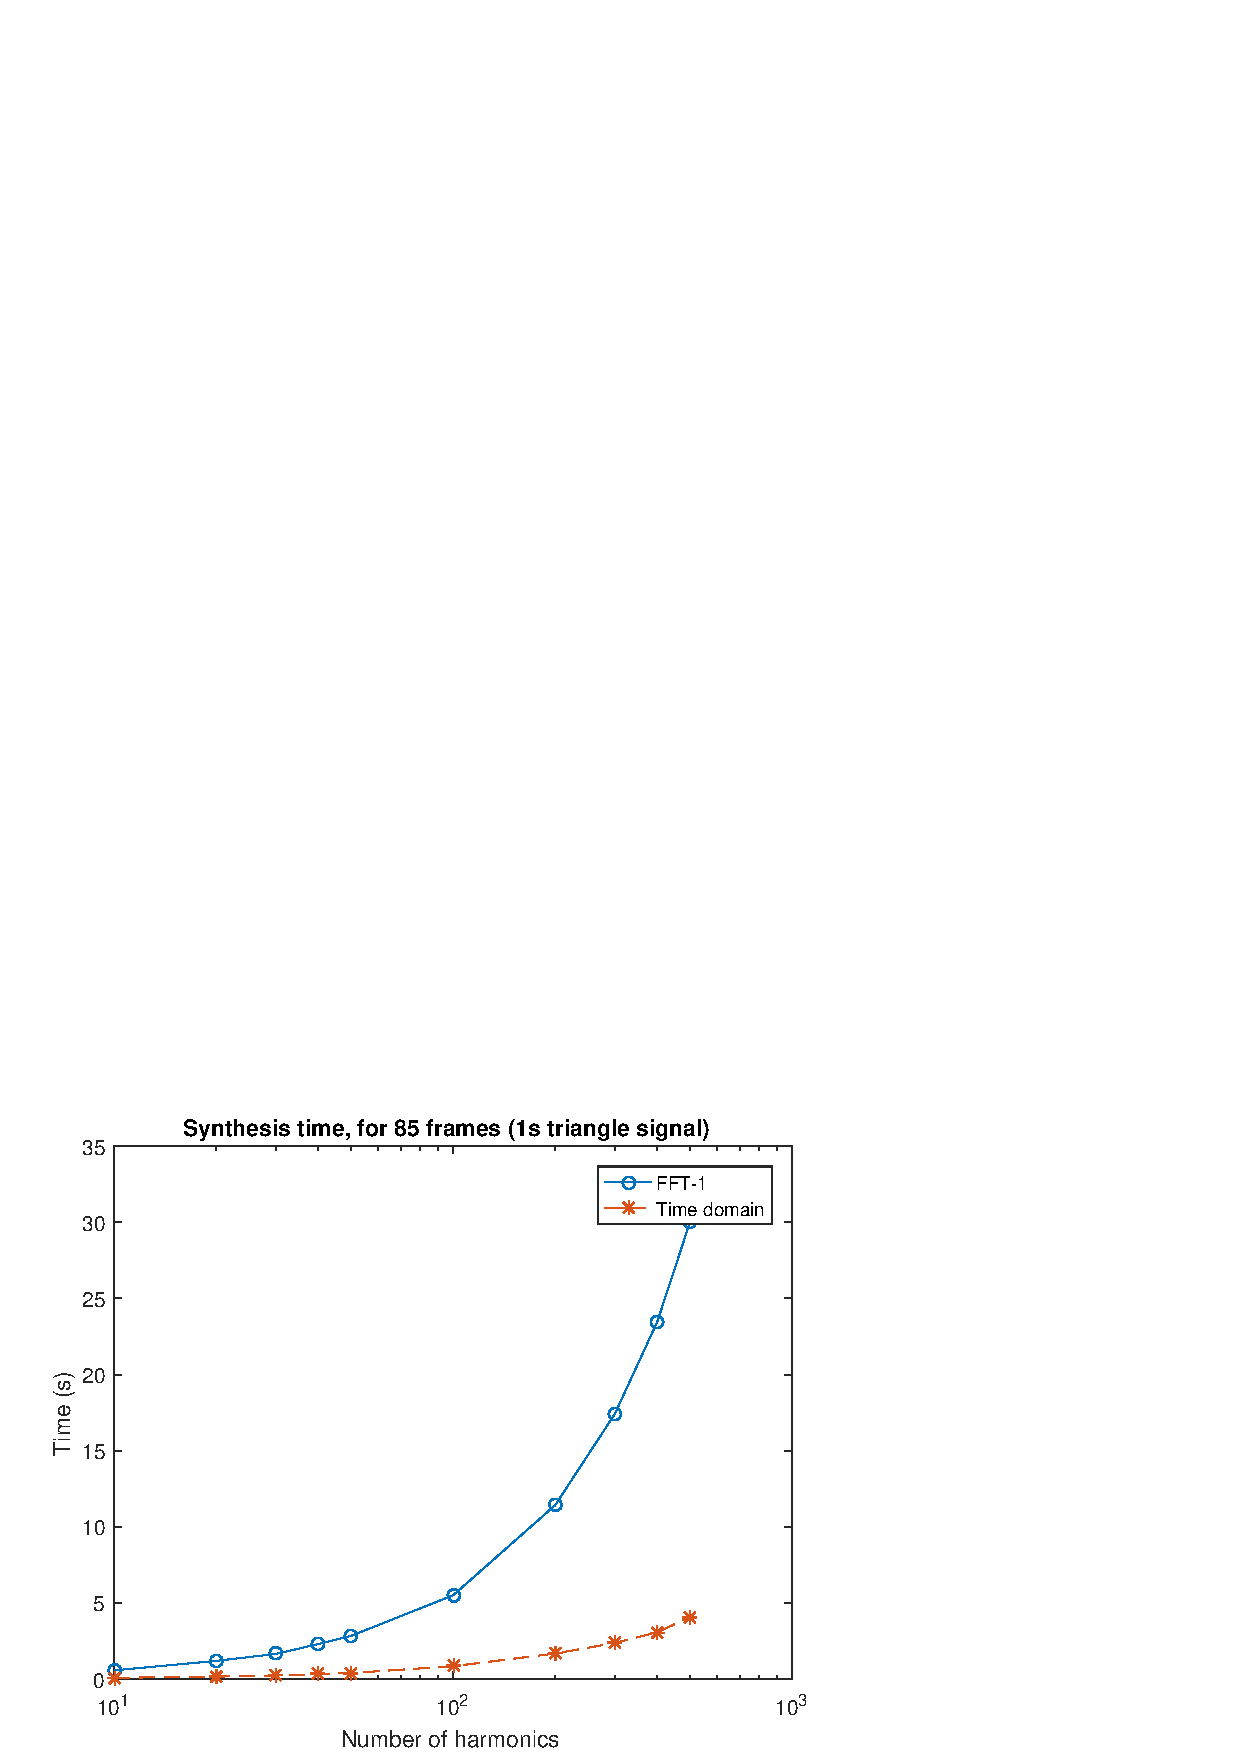
\includegraphics[scale=0.4]{time.pdf}
      \caption{\it Time of execution}
   \end{minipage} \hfill
   \begin{minipage}[c]{.46\linewidth}
      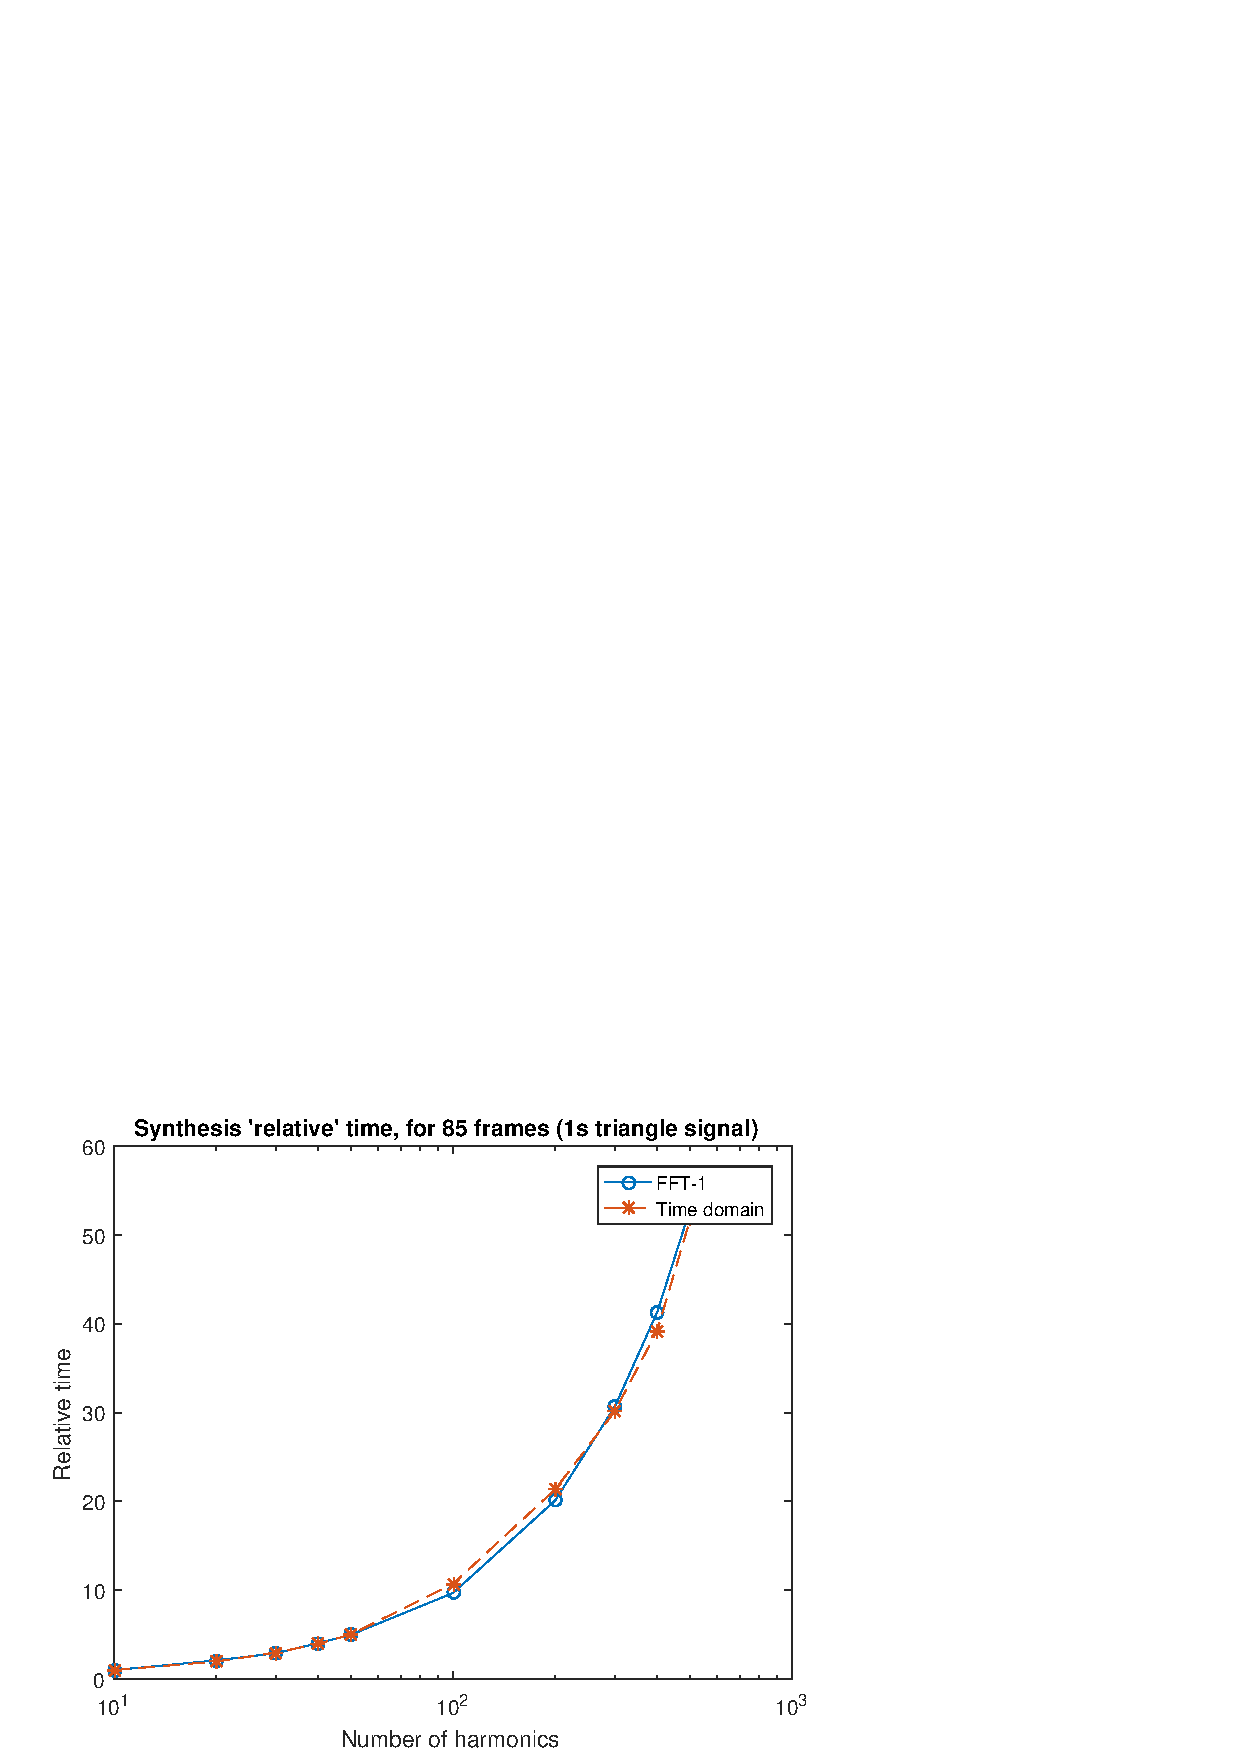
\includegraphics[scale=0.4]{relativetime.pdf}
      \caption{\it Relative Time of Execution}
   \end{minipage}
\end{figure}
\end{frame}
%-------------------------------------------------------
\begin{frame}{Stationary Case}{RMSE}
%-------------------------------------------------------
\begin{figure}
      \includegraphics[scale=0.4]{rmse.pdf}
      \caption{\it RMSE (original vs. synthesized triangular wave}
\end{figure}
\end{frame}
%-------------------------------------------------------
\subsection{Non-Stationary Case}
\begin{frame}{Non-Stationary Case}{Chirps}
%-------------------------------------------------------

The idea is to try the method on some chirps signal. And then on real sounds, like instruments and voices.

\begin{figure}
{\includegraphics[scale=0.45]{chirps.png}}
	\caption{\it Chirp signal to test}
\end{figure}
We can measure the error of the lobe interpolation with the Look-Up Table. (Not done)
\end{frame}

%%%%%%%%%%%%%%%%%
%-------------------------------------------------------
\section{Conclusion}
%-------------------------------------------------------
\subsection{Conclusion}
\begin{frame}{Conclusion}{}
%-------------------------------------------------------
\begin{itemize}
\item 6 weeks only
\medskip
\item Research subject $\Rightarrow$ Can it really works ?
\medskip
\item Lots of trouble when we try to understand the phase coherence problem
\medskip
\end{itemize}
\centering
\medskip
\medskip
\medskip
\medskip
\medskip
\Large Do you have any question?
\end{frame}
%-------------------------------------------------------
\subsection{References}
\begin{frame}{References}{}
%-------------------------------------------------------
\begin{itemize}
\justifying
	\item Jeremy G. Wells, Damian T. Murphy \og High accuracy frame-by-frame
	non-stationary modelling,\fg , Audio Lab, Intelligent Systems Group,
	Department of Electronics, University of York, YO10 5DD, UK,
	September 2006.
	
	\item Jeremy J. Wells, \og Methods dor separation of amplitude and fequency
	modulation in Fourier transformed signals\fg, AudioLab, Department of
	Electronics, September 2010.
	
	\item D. Brandon Lloyd, Ninkunj Raghuvanshi, Naga K. Govindaraju, \og Sound
	synthesis for impact sounds in videogames\fg, eXtrem computing group,
	Microsoft research, 2011.
	
	\item Thorsten Karrer, Eric Lee, Jan Borchers, \og A phase vocoder for real-time
	time-stretching\fg, Media computing group.

\end{itemize}

\end{frame}



\end{document}
